\section{Introduction to Object Detection}
\begin{frame}{}
    \LARGE Object Detection: \textbf{Introduction}
\end{frame}

\begin{frame}[allowframebreaks]{Object Detection}
    \begin{figure}
        \centering
        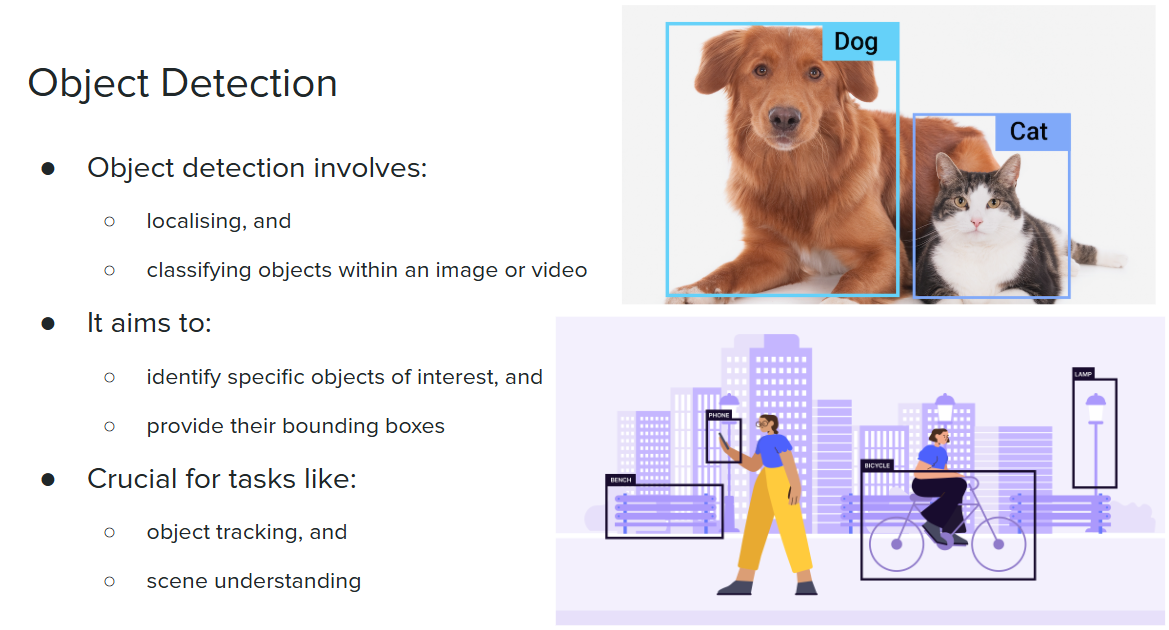
\includegraphics[width=1.02\textwidth,height=0.9\textheight,keepaspectratio]{images/object-detect/intro-1.png}
    \end{figure}

\framebreak

    \begin{itemize}
        \item \textbf{Input:} Single RGB Image
        \item \textbf{Output:} A set of detected objects. For each object predict:
        \begin{itemize}
            \item Category label (from fixed, known set of categories)
            \item Bounding box (four numbers: x, y, width, height)
        \end{itemize}
    \end{itemize}

\framebreak

    \begin{figure}
        \centering
        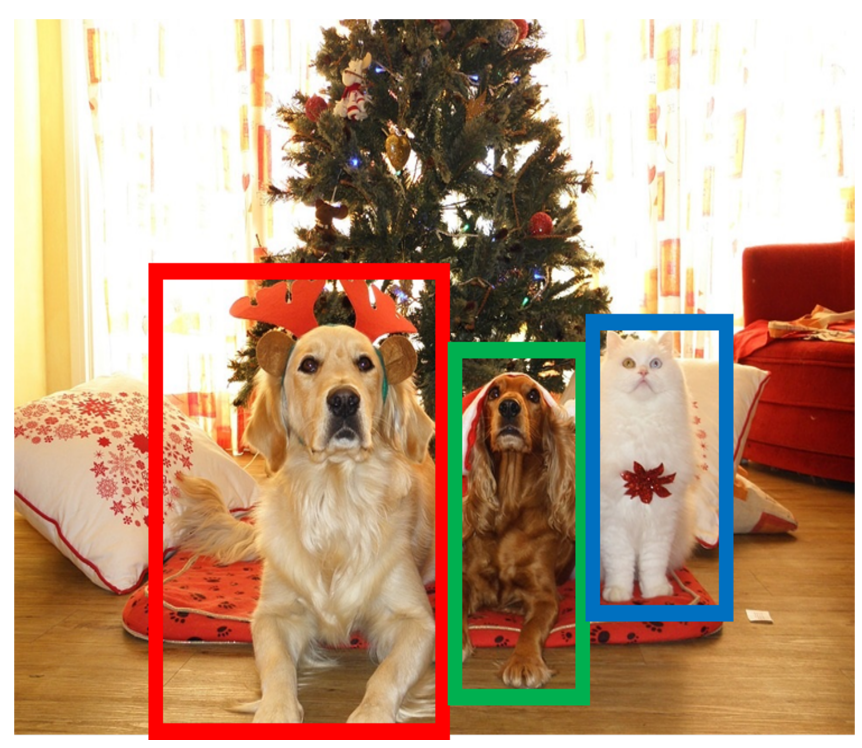
\includegraphics[width=1.0\textwidth,height=0.95\textheight,keepaspectratio]{images/object-detect/object_1.png}
    \end{figure}

\framebreak

    \begin{figure}
        \centering
        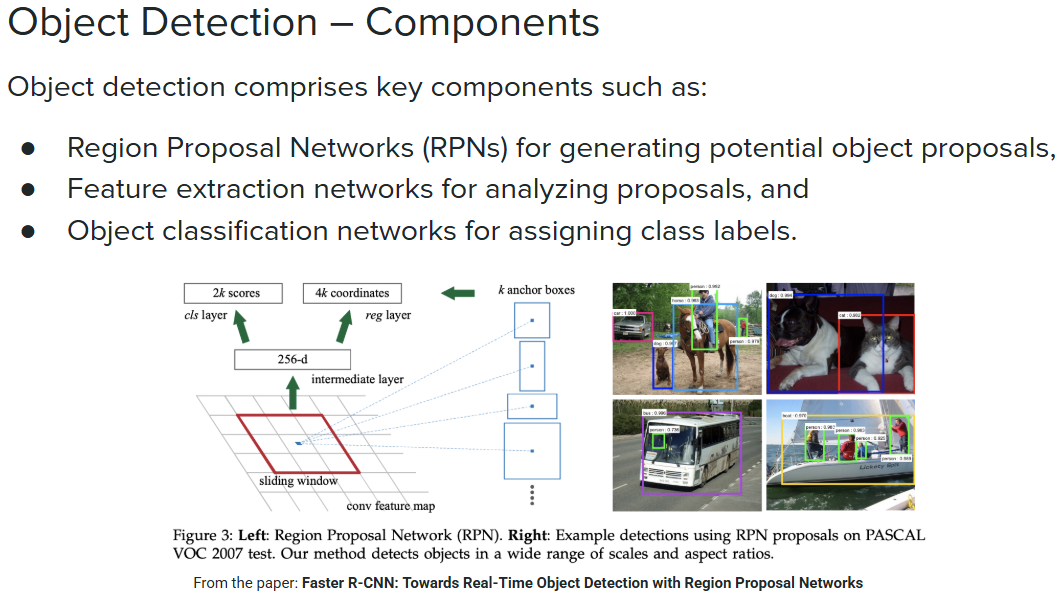
\includegraphics[width=1.02\textwidth,height=0.9\textheight,keepaspectratio]{images/object-detect/intro-2.png}
    \end{figure}

\framebreak

    \begin{figure}
        \centering
        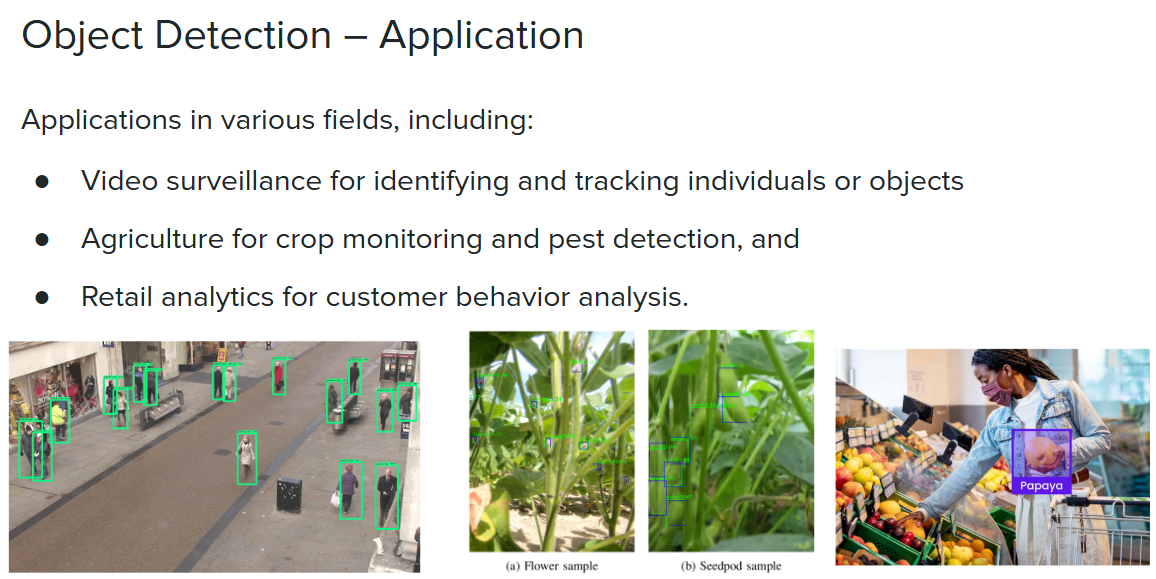
\includegraphics[width=1.02\textwidth,height=0.9\textheight,keepaspectratio]{images/object-detect/intro-3.png}
    \end{figure}
    
\end{frame}

\begin{frame}{Object Detection: Challenges}
    \begin{itemize}
        \item \textbf{Multiple outputs:} Need to output variable numbers of objects per image
        \item \textbf{Multiple types of output:} Need to predict "what" (category label) as well as "where" (bounding box)
        \item \textbf{Large images:} Classification works at 224x224; need higher resolution for detection, often $\sim 800 \times 600$
    \end{itemize}
\end{frame}

